\documentclass[utf8,russian]{beamer}
\mode<presentation> {
  \usetheme{Madrid}
}

\usepackage{graphicx}
\usepackage{booktabs}
\usepackage{listings}
\usepackage[utf8]{inputenc}
\usepackage[T2A]{fontenc}
\usepackage[russian,english]{babel}

\setbeamertemplate{navigation symbols}{}

\setbeamercolor{footline}{}
\setbeamertemplate{footline}{
  \leavevmode%
  \hbox{
  \begin{beamercolorbox}[wd=.333333\paperwidth,ht=2.25ex,dp=1ex,center]{}%
    Н. М. Нежевский (Мехмат ЮФУ)
  \end{beamercolorbox}%
  \begin{beamercolorbox}[wd=.333333\paperwidth,ht=2.25ex,dp=1ex,center]{}%
    Ростов-на-Дону, 2016
  \end{beamercolorbox}%
  \begin{beamercolorbox}[wd=.333333\paperwidth,ht=2.25ex,dp=1ex,right]{}%
  Стр. \insertframenumber{} из \inserttotalframenumber \hspace*{2ex}
  \end{beamercolorbox}}%
  \vskip0pt%
}

\title{\small{Цветовая поддержка вывода консоли интерпретатора языка Haskell GHCi}}
\vspace{15pt}%
\author{\small{%
Н. М. Нежевский\\%
\emph{Направление подготовки:}~Фундаментальная информатика и \\информационные технологии\\%
\emph{Научный руководитель:} старший преподаватель В.~Н.~Брагилевский}\\%
\vspace{15pt}%
    Южный федеральный университет\\
    Институт математики, механики и компьютерных наук
    имени~И.\,И.\,Воровича%
}
\date{\small{Ростов-на-Дону, 2016}}

\begin{document}

\begin{frame}
\titlepage
\end{frame}

\begin{frame}
\frametitle{Содержание}
\tableofcontents
\end{frame}

\section{Постановка задачи}
\begin{frame}
\frametitle{Постановка задачи}
\begin{itemize}
  \item Анализ возможных подходов к реализации подсветки вывода
  \item Изучение программной структуры GHCi
  \item Программная реализация цветовой поддержки вывода интерпретатора GHCi
\end{itemize}
\end{frame}

\section{Программная реализация}
\begin{frame}
\frametitle{Программная реализация}

\begin{block}{Реализация на основе внешней обработки}
Получена программная реализация, обрабатывающая консольный вывод GHCi
\end{block}

\begin{block}{Алгоритм работы}
\begin{enumerate}
  \item Внешняя программа-обработчик принимает пользовательский ввод
  \item Этот пользовательский ввод передаётся в GHCi
  \item Программа-обработчик перехватывает результат вывода GHCi
  \item Строковый вывод окрашивается добавлением ANSI символов и возвращается пользователю
\end{enumerate}
\end{block}
\end{frame}
\begin{frame}{Пример использования}
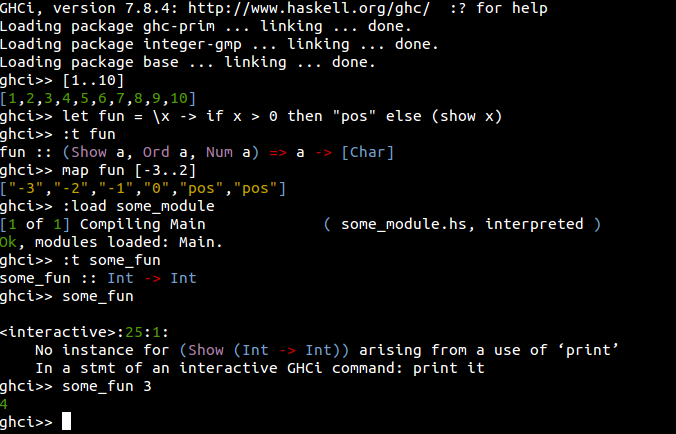
\includegraphics[scale=0.5]{img/example.png}
\end{frame}


\onslide<1>
\begin{frame}{Анализ полученной реализации}

\begin{block}{Недостатки реализации}

  \begin{enumerate}
    \item Окрашивание возможно только для стандартных типов и классов типов
    \item Не поддерживается окрашивание переменных
  \end{enumerate}
\end{block}

\onslide<2>

\begin{block}{Вывод}
Полученная реализация решает поставленную задачу, однако имеет ряд ограничений
\end{block}

\end{frame}

\section{Система печати в GHC}

\begin{frame}[fragile]
\frametitle{Система вывода в GHC}
\begin{block}{Система печати}
Система печати в GHC основана на принципе структурной печати
\end{block}

\begin{block}{Используемые типы}
Тип Doc является примитивом структурной печати
\begin{lstlisting}[language=Haskell]
data Doc
 = Empty
 | NilAbove Doc
 | Nest FastInt Doc
 | Union Doc Doc
 | ...
\end{lstlisting}
\end{block}
\end{frame}

\begin{frame}[fragile]
\frametitle{SDoc и Outputable}

\begin{block}{Тип SDoc}
Тип SDoc является обёрткой над типом Doc. Он содержит дополнительную информацию для печати
\begin{lstlisting}[language=Haskell]
type SDoc = PprStyle -> Doc
\end{lstlisting}
\end{block}

\begin{block}{Класс типов Outputable}
Класс типов Outputable предоставляет интерфейс для типов, поддерживающих функцию структурной печати.
\begin{lstlisting}[language=Haskell]
class Outputable a where
	ppr :: a -> SDoc
\end{lstlisting}
\end{block}

\end{frame}

\begin{frame}[fragile]
\frametitle{Изменения в модуле Outputable}

\begin{block}{Модель печати}
Была разработана модель печати, аналогичная модели в GHCi, по которой были выведены необходимые изменения
\end{block}

\begin{block}{Изменение типа SDoc}
В обёртку над типом Doc добавлена информация о цвете
\begin{lstlisting}[language=Haskell]
type SDoc = SDocStyle -> Doc
data SDocStyle = {
    pprStyle :: PprStyle,
    pprColor :: PprColor
}
\end{lstlisting}
\end{block}
\end{frame}

\begin{frame}[fragile]
\frametitle{Класс типов ColorOutputable}

\begin{block}{ColorOutputable}
Создан класс типов ColorOutputable, предоставляющий интерфейс для печати с подсветкой
\begin{lstlisting}[language=Haskell]
class Outputable a => ColorOutputable a where
  cppr :: a -> SDoc
\end{lstlisting}
\end{block}

\begin{block}{}
Для полной поддержки введённых изменений необходимо заменить Outputable на ColorOutputable
\end{block}

\end{frame}

\begin{frame}[fragile]
\frametitle{Пример внедрения изменений}

\begin{block}{}
На основе изменений в качестве примера была переработана mkExpectedActualMsg
\end{block}

\begin{block}{Изменённая функция mkExpectedActualMsg}
\begin{lstlisting}
mkExpectedActualMsg :: Type -> Type -> SDoc
mkExpectedActualMsg exp_ty act_ty
  = vcat [ colorize cRed $ ptext 
         (text "Expected type:") <+> cppr exp_ty
         , colorize cRed $ ptext 
         (text "  Actual type:") <+> cppr act_ty]
\end{lstlisting}
\end{block}

\end{frame}

\section{Полученные результаты}
\begin{frame}{Полученные результаты}
\begin{itemize}
  \item Создана программная реализация, частично решающая поставленную задачу
  \item Получен список необходимых изменений для встроенной поддержки подсветки вывода
\end{itemize}
\end{frame}

\end{document}